\section{基本可行解}
\label{sec:lp-basic-solutions}

线性规划的最优解是否一定落在角点上，角点又怎样用矩阵计算出来？车间问题里这一点靠眼睛看到，变量多了就要靠下面的定义和定理。

\paragraph{多面体与极点}
车间的四边形由四个半平面相交而成。一般地，满足$\bm{g}\neq\bm{0}$的集合$\{\bm{x}:\bm{g}^\top\bm{x}\leq h\}$称为\term{半空间}（halfspace），有限个半空间的交称为\term{多面体}（polyhedron）。写成矩阵形式，就是
\begin{equation}
 \bm{Q}=\{\bm{x}\in\mathbb{R}^n:\bm{G}\bm{x}\leq\bm{h}\},
 \label{eq:lp-polyhedron}
\end{equation}
其中$\bm{G}$的行数有限。等式可以写成两条方向相反的不等式，所以标准型的可行集$\bm{C}$也是多面体。半空间是闭凸集，有限个闭凸集的交仍是闭凸集，多面体因此是闭凸集。

“角点”需要一个不依赖图形的说法。观察图~\ref{fig:lp-extreme-midpoint}：内部的点是某条可行线段的中点，边上的点也是，只不过线段只能沿边摆放。顶点不同，过它的线段无论怎么摆，总有一端跑到可行集外面。

\begin{BookInlineFigure}
 \centering
 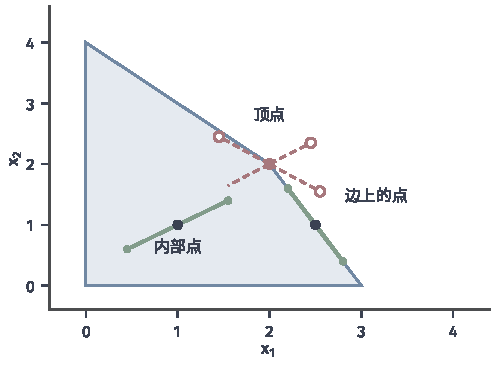
\includegraphics[width=84mm]{figures/05-optimization/01-linear-programming/matplotlib/lp-extreme-midpoint/figure.pdf}
 \caption{三种位置的点。深色的内部点和边上的点都是一条可行线段（绿色）的中点。红点$(2,2)$是顶点，过它的线段（红色虚线）总有一端落在四边形外（空心点），所以它不是任何可行线段的中点。}
 \label{fig:lp-extreme-midpoint}
\end{BookInlineFigure}

\begin{definition}[极点]
 \label{def:lp-extreme-point}
 设$\bm{Q}$是凸集，$\bm{x}\in\bm{Q}$。若$\bm{u},\bm{v}\in\bm{Q}$且$\bm{x}=(\bm{u}+\bm{v})/2$只有在$\bm{u}=\bm{v}=\bm{x}$时才成立，就称$\bm{x}$是$\bm{Q}$的\term{极点}（extreme point）。
\end{definition}

对多面体，极点也称为顶点，本章两种说法通用。

\paragraph{基与基本解}
标准型的可行点要满足$m$个等式，却有$n$个未知数，还剩$n-m$个自由度。平面上的顶点是让两条约束同时取等号得到的，在标准型里，取等号的办法是让坐标变成零。于是自然的做法是：让$n-m$个坐标取零，用$m$个等式解出其余$m$个坐标。

能否解出，取决于留下的那$m$列是否线性无关。

\begin{definition}[基与基本可行解]
 \label{def:lp-basic-solution}
 设$\bm{A}$满行秩。取$m$个下标组成集合$B$，其余下标组成$N$。若由$B$中各列构成的方阵$\bm{A}_B$可逆，就称$B$为一个基，$\bm{A}_B$为\term{基矩阵}（basis matrix）。令
 \begin{equation}
  \bm{x}_B=\bm{A}_B^{-1}\bm{b},\qquad\bm{x}_N=\bm{0},
  \label{eq:lp-basic-solution}
 \end{equation}
 所得的$\bm{x}$称为基$B$对应的\term{基本解}（basic solution），$\bm{x}_B$和$\bm{x}_N$的分量分别称为基分量和非基分量。若还有$\bm{x}_B\geq\bm{0}$，就称$\bm{x}$为\term{基本可行解}（basic feasible solution），$B$为可行基。
\end{definition}

基本解满足全部等式，但不一定非负，所以不一定可行。在车间问题~\eqref{eq:lp-workshop-standard}中，$\bm{A}$的四列任取两列都线性无关，共有$\binom{4}{2}=6$个基。以$B=\{1,4\}$为例，令$x_2=x_3=0$，两个等式变成
\[
 x_1=4,\qquad 2x_1+x_4=6.
\]
解得$x_1=4$，$x_4=-2$。分量为负，这个基本解不可行：产量$(4,0)$用掉的原料比库存多$2$。表~\ref{tab:lp-six-bases}列出了全部六个基本解。

\begin{BookInlineTable}
 \centering
 \begin{tabular}{cccc}
  \toprule
  基$B$ & $\bm{x}=(x_1,x_2,x_3,x_4)$ & 平面上的点 & 是否可行\\
  \midrule
  $\{3,4\}$ & $(0,0,4,6)$ & $(0,0)$ & 可行\\
  $\{1,3\}$ & $(3,0,1,0)$ & $(3,0)$ & 可行\\
  $\{2,4\}$ & $(0,4,0,2)$ & $(0,4)$ & 可行\\
  $\{1,2\}$ & $(2,2,0,0)$ & $(2,2)$ & 可行\\
  $\{1,4\}$ & $(4,0,0,-2)$ & $(4,0)$ & 不可行\\
  $\{2,3\}$ & $(0,6,-2,0)$ & $(0,6)$ & 不可行\\
  \bottomrule
 \end{tabular}
 \caption{车间问题的六个基本解。可行的四个恰好是四边形的四个顶点。}
 \label{tab:lp-six-bases}
\end{BookInlineTable}

图~\ref{fig:lp-basic-solutions}把这六个点画在平面上。它们正是四条边界直线的两两交点：选定基，就是选定哪两个坐标取零，也就是选定哪两条边界同时取等号。

\begin{BookInlineFigure}
 \centering
 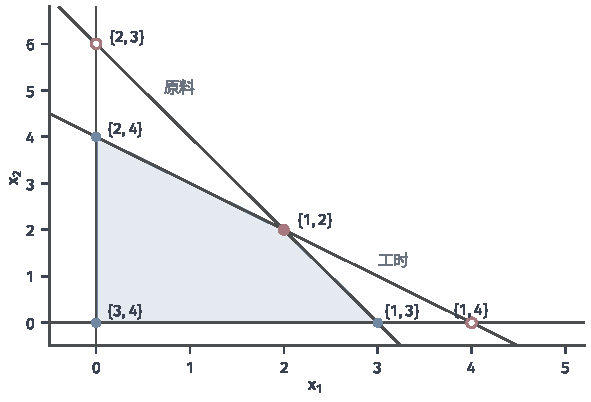
\includegraphics[width=100mm]{figures/05-optimization/01-linear-programming/matplotlib/lp-basic-solutions/figure.pdf}
 \caption{车间问题的六个基本解，点旁标出对应的基。四条直线是$x_1=0$、$x_2=0$和工时、原料两条约束的边界。实心点是四个基本可行解，其中红点$(2,2)$最优；红色空心点$(4,0)$和$(0,6)$的基本解有负分量，落在可行域外。}
 \label{fig:lp-basic-solutions}
\end{BookInlineFigure}

\paragraph{基本可行解就是极点}
表中四个可行的基本解恰好是四个顶点，这不是巧合。下面的定理把代数对象和几何对象连起来，判别的依据是矩阵的秩：只看正分量所在的列。

\begin{theorem}[基本可行解与极点]
 \label{thm:lp-bfs-extreme}
 设$\bm{A}$满行秩，$\bm{x}\in\bm{C}$，$J=\{j:x_j>0\}$。下面三条等价：
 \begin{enumerate}
  \item $\bm{x}$是$\bm{C}$的极点；
  \item 列$\{\bm{a}_j:j\in J\}$线性无关；
  \item $\bm{x}$是某个基对应的基本可行解。
 \end{enumerate}
\end{theorem}

\begin{proof}
 先证(1)推出(2)。假设这些列线性相关，则有不全为零的系数$w_j$（$j\in J$）使$\sum_{j\in J}w_j\bm{a}_j=\bm{0}$。把$\bm{w}$在$J$以外的分量补成零，就有
 \[
  \bm{A}\bm{w}=\bm{0},\qquad\bm{w}\neq\bm{0}.
 \]
 $J$上的$x_j$都是正数，取足够小的$\varepsilon>0$，可使$\bm{x}\pm\varepsilon\bm{w}\geq\bm{0}$。再由$\bm{A}\bm{w}=\bm{0}$知这两个点都满足等式，都可行。它们不相等，而$\bm{x}$是它们的中点，与$\bm{x}$是极点矛盾。

 再证(2)推出(3)。线性无关的列不超过$m$个，所以$\lvert J\rvert\leq m$。$\bm{A}$满行秩，它的列张成$\mathbb{R}^m$，可以再补入若干列，把$\{\bm{a}_j:j\in J\}$扩充成$\mathbb{R}^m$的一组基，相应的下标集记为$B\supseteq J$。于是$\bm{A}_B$可逆，$B$之外的分量都不在$J$中，所以$\bm{x}_N=\bm{0}$。代入等式得到
 \[
  \bm{A}_B\bm{x}_B=\bm{b},\qquad\text{即}\qquad\bm{x}_B=\bm{A}_B^{-1}\bm{b}.
 \]
 又$\bm{x}$可行，故$\bm{x}_B\geq\bm{0}$，它是基$B$的基本可行解。

 最后证(3)推出(1)。设$\bm{x}$是基$B$的基本可行解，且$\bm{x}=(\bm{u}+\bm{v})/2$，$\bm{u},\bm{v}\in\bm{C}$。对$j\in N$，有$u_j+v_j=2x_j=0$，又$u_j,v_j\geq0$，所以$u_j=v_j=0$。于是$\bm{A}_B\bm{u}_B=\bm{b}$，由$\bm{A}_B$可逆得到
 \[
  \bm{u}_B=\bm{A}_B^{-1}\bm{b}=\bm{x}_B.
 \]
 所以$\bm{u}=\bm{x}$，同理$\bm{v}=\bm{x}$。
\end{proof}

定理中的秩条件有直接的几何解释。在点$\bm{x}$处取等号的约束是$m$个等式和$n-\lvert J\rvert$个“坐标为零”。把它们的系数排成矩阵$\bm{M}$，$\bm{M}\bm{v}=\bm{0}$说的是
\[
 \bm{v}_{J^c}=\bm{0},\qquad\bm{A}_J\bm{v}_J=\bm{0}.
\]
其中$J^c$是$J$的补集。所以$\bm{M}$的列满秩，也就是取等号的约束能唯一确定一个点，当且仅当$\bm{A}_J$的列线性无关。“$n$个线性无关的约束取等号”和“基矩阵可逆”是同一件事的两种说法。

用车间问题验证一下。点$(5/2,1)$对应$\bm{x}=(5/2,1,1/2,0)^\top$，正分量在第$1,2,3$列，三列放在$\mathbb{R}^2$中线性相关，取
\[
 \bm{w}=(-1,2,-1,0)^\top,\qquad\bm{A}\bm{w}=\bm{0}.
\]
$\bm{x}\pm\varepsilon\bm{w}$都可行，所以它不是极点，在图上它是原料边界中间的一点。点$(2,2)$对应$\bm{x}=(2,2,0,0)^\top$，第$1,2$列线性无关，它是极点。

基的个数不超过$\binom{n}{m}$，所以极点只有有限个。最优解若能在极点取得，问题就从无穷多个候选变成了有限多个。

\paragraph{最优解可以在基本可行解中取得}
下面证明这确实成立。证明的想法很具体：任取一个可行点，如果它的正分量对应的列线性相关，就有一个方向可以沿着走，目标不变差，直到某个正分量降到零。正分量越来越少，最后得到一个基本可行解。

\begin{lemma}[推向基本可行解]
 \label{lem:lp-push}
 设$\bm{A}$满行秩，且$\bm{c}^\top\bm{x}$在$\bm{C}$上有下界。则对每个$\bm{x}\in\bm{C}$，存在基本可行解$\widehat{\bm{x}}$，使
 \begin{equation}
  \bm{c}^\top\widehat{\bm{x}}\leq\bm{c}^\top\bm{x}.
  \label{eq:lp-push}
 \end{equation}
\end{lemma}

\begin{proof}
 对正分量的个数$\lvert J\rvert$归纳。若列$\{\bm{a}_j:j\in J\}$线性无关，由定理~\ref{thm:lp-bfs-extreme}，$\bm{x}$本身就是基本可行解。

 否则取$\bm{w}\neq\bm{0}$，满足$\bm{A}\bm{w}=\bm{0}$，且$w_j=0$对$j\notin J$成立。必要时用$-\bm{w}$代替$\bm{w}$，可使$\bm{c}^\top\bm{w}\leq0$。先说明可以假设$\bm{w}$有负分量。

 若$\bm{w}\geq\bm{0}$且$\bm{c}^\top\bm{w}<0$，则对一切$t\geq0$，点$\bm{x}+t\bm{w}$可行，目标值$\bm{c}^\top\bm{x}+t\bm{c}^\top\bm{w}$趋于$-\infty$，与有下界矛盾，这种情形不出现。若$\bm{w}\geq\bm{0}$且$\bm{c}^\top\bm{w}=0$，就把$\bm{w}$换成$-\bm{w}$，此时$\bm{c}^\top\bm{w}$仍为零，而$\bm{w}$有了负分量。

 现在令
 \[
  t^\star=\min_{j:\,w_j<0}\frac{x_j}{-w_j},\qquad\bm{x}'=\bm{x}+t^\star\bm{w}.
 \]
 负分量只出现在$J$中，那里$x_j>0$，所以$t^\star>0$。$t^\star$的取法保证$\bm{x}'\geq\bm{0}$，又$\bm{A}\bm{x}'=\bm{b}$，所以$\bm{x}'$可行，并且
 \[
  \bm{c}^\top\bm{x}'=\bm{c}^\top\bm{x}+t^\star\bm{c}^\top\bm{w}\leq\bm{c}^\top\bm{x}.
 \]

 $J$之外的分量保持为零，取到最小值的分量变成零，所以$\bm{x}'$的正分量个数严格减少。对$\bm{x}'$用归纳假设，即得$\widehat{\bm{x}}$。
\end{proof}

用车间问题走一遍。从可行点$(x_1,x_2)=(1,1)$出发，四个坐标是$\bm{x}=(1,1,2,3)^\top$，目标值$-5$。四列放在$\mathbb{R}^2$中必然线性相关，可以取下面的方向，并算出步长：
\[
 \bm{w}=(1,0,-1,-2)^\top,\qquad\bm{c}^\top\bm{w}=-3,\qquad
 t^\star=\min\Bigl\{\frac{2}{1},\frac{3}{2}\Bigr\}=\frac32.
\]
走完得到第一个新点，$x_4$降到了零：
\[
 \bm{x}'=\Bigl(\frac52,1,\frac12,0\Bigr)^\top,\qquad\bm{c}^\top\bm{x}'=-\frac{19}{2}.
\]

此时还剩三个正分量，第$1,2,3$列在$\mathbb{R}^2$中仍然线性相关。满足$w_4=0$的零空间方向是$(1,-2,1,0)^\top$，它的目标变化率是$+1$，所以取反方向，并求步长：
\[
 \bm{w}=(-1,2,-1,0)^\top,\qquad\bm{c}^\top\bm{w}=-1,\qquad
 t^\star=\min\Bigl\{\frac{5/2}{1},\frac{1/2}{1}\Bigr\}=\frac12.
\]
走完得到
\[
 \bm{x}''=(2,2,0,0)^\top,\qquad\bm{c}^\top\bm{x}''=-10.
\]
正分量只剩两个，对应的列线性无关，这就是基本可行解。图~\ref{fig:lp-push-to-vertex}显示了这两步：先水平走到原料边界，再沿边界走到顶点。这里碰巧到达了最优解，一般只能保证目标不变差。

\begin{BookInlineFigure}
 \centering
 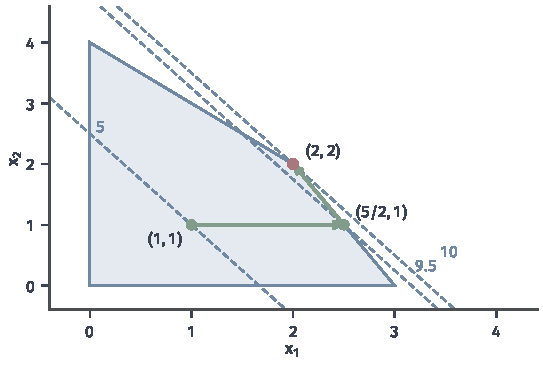
\includegraphics[width=92mm]{figures/05-optimization/01-linear-programming/matplotlib/lp-push-to-vertex/figure.pdf}
 \caption{引理~\ref{lem:lp-push}在车间问题上的两步。绿色箭头从$(1,1)$（四个正分量）走到$(5/2,1)$（三个正分量），再走到顶点$(2,2)$（两个正分量）。蓝色虚线是利润等于$5$、$9.5$、$10$的等值线，每一步都不使利润变小。}
 \label{fig:lp-push-to-vertex}
\end{BookInlineFigure}

\begin{theorem}[最优基本可行解的存在]
 \label{thm:lp-optimal-bfs}
 设$\bm{A}$满行秩。若标准型~\eqref{eq:lp-standard}可行且最优值有限，则最优值能够取到，并且至少有一个最优解是基本可行解。特别地，非空的$\bm{C}$至少有一个极点。
\end{theorem}

\begin{proof}
 基本可行解至多有$\binom{n}{m}$个，由引理~\ref{lem:lp-push}（对$\bm{C}$中任一点使用），它们至少有一个。在这有限个点中取目标值最小的$\bm{x}^\star$。对任意$\bm{x}\in\bm{C}$，引理给出基本可行解$\widehat{\bm{x}}$，于是
 \[
  \bm{c}^\top\bm{x}\geq\bm{c}^\top\widehat{\bm{x}}\geq\bm{c}^\top\bm{x}^\star.
 \]
 所以$\bm{x}^\star$是最优解。最后一句取$\bm{c}=\bm{0}$即得。
\end{proof}

定理中“$\bm{A}$满行秩”只是为了让基有定义，这一点上一节已经保证。这个结论比一般的存在定理强。第~\ref{chap:optimization}章的$e^x$有下界却取不到下确界，而标准型线性规划只要最优值有限，就一定取得到，并不要求可行集有界。条件里的“可行”和“最优值有限”各自排除一种结局，图~\ref{fig:lp-three-outcomes}画出了线性规划的三种情形。

\begin{BookInlineFigure}
 \centering
 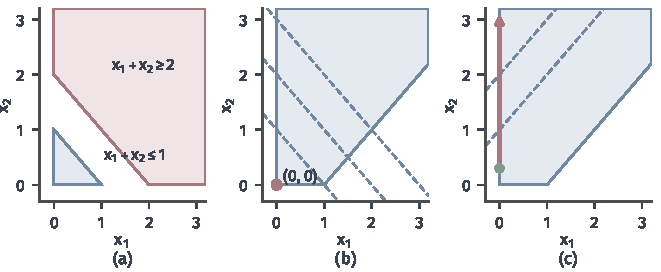
\includegraphics[width=112mm]{figures/05-optimization/01-linear-programming/matplotlib/lp-three-outcomes/figure.pdf}
 \caption{线性规划的三种结局。(a)~第一象限中两条约束围成的区域不相交，问题不可行。(b)~可行域$\{\bm{x}\geq\bm{0},\ x_1-x_2\leq1\}$无界，但最小化$x_1+x_2$（蓝色虚线是等值线）的最优解存在，是红点$(0,0)$。(c)~同一可行域上最小化$x_1-x_2$，从绿点沿红色射线一直走，目标趋于$-\infty$，问题无下界。}
 \label{fig:lp-three-outcomes}
\end{BookInlineFigure}

定理只说有一个最优解是基本可行解，不说所有最优解都是。把车间的目标改成最大化$2x_1+x_2$，等值线与原料边界平行，图~\ref{fig:lp-optimal-face}(b)中$(2,2)$和$(3,0)$都最优，它们连线上的每一点也都最优。中点$(5/2,1)$对应$\bm{x}=(5/2,1,1/2,0)^\top$，有三个正分量，多于$m=2$，所以不是基本可行解，却同样最优。

\begin{BookInlineFigure}
 \centering
 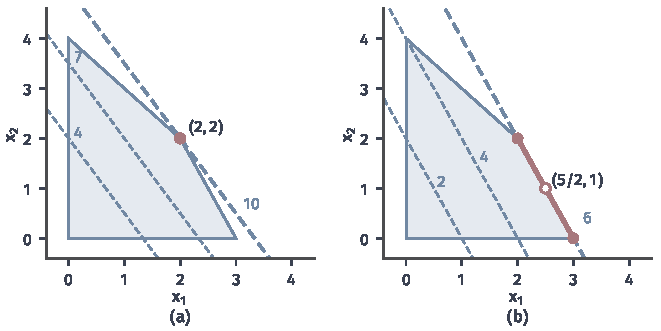
\includegraphics[width=112mm]{figures/05-optimization/01-linear-programming/matplotlib/lp-optimal-face/figure.pdf}
 \caption{等值线平移到最后接触可行域的情形。(a)~最大化$3x_1+2x_2$，粗虚线（利润$10$）只接触顶点$(2,2)$，最优解唯一。(b)~最大化$2x_1+x_2$，粗虚线（值为$6$）与一条边重合，红色线段上都是最优解，其中空心点$(5/2,1)$不是顶点。}
 \label{fig:lp-optimal-face}
\end{BookInlineFigure}

定理把问题化成了有限比较，但枚举全部的基并不现实。$n=100$，$m=50$时，$\binom{n}{m}$约为$1.0\times10^{29}$。需要的是一种不逐个检查、只在相邻顶点之间移动的办法，下面先说清“相邻”是什么意思。

\paragraph{沿边到相邻顶点}
在车间的四边形上，相邻顶点由一条边相连。用基来说，相邻的两个基只差一个下标。设$B$是可行基，$\bar{\bm{x}}$是它的基本可行解，取一个不在$B$中的下标$q$。让$x_q$从零增大，其余非基分量保持为零，基分量必须随之调整，以维持等式。由$\bm{A}_B\bm{x}_B+\bm{a}_qx_q=\bm{b}$解出
\begin{equation}
 \bm{x}_B=\bar{\bm{x}}_B-x_q\bm{u},\qquad\bm{u}=\bm{A}_B^{-1}\bm{a}_q.
 \label{eq:lp-edge-direction}
\end{equation}
这相当于让点沿方向$\bm{d}$移动，其中$d_q=1$，$\bm{d}_B=-\bm{u}$，其余分量为零，并且$\bm{A}\bm{d}=\bm{0}$。

\begin{theorem}[沿边的移动]
 \label{thm:lp-edge-move}
 设$\bm{A}$满行秩，$B$是可行基，$\bar{\bm{x}}$是其基本可行解，$q\notin B$，$\bm{u}$和$\bm{d}$如上。则满足“$x_j=0$对$j\notin B\cup\{q\}$成立”的可行点恰好是$\bar{\bm{x}}+\alpha\bm{d}$，其中$\alpha\geq0$且$\bar{\bm{x}}_B-\alpha\bm{u}\geq\bm{0}$。进一步：
 \begin{enumerate}
  \item 若$\bm{u}$有正分量，且$\bar{\bm{x}}_B>\bm{0}$，记$r$是下式取到最小值的位置，$B(i)$是基中第$i$个下标：
  \begin{equation}
   \alpha^\star=\min_{i:\,u_i>0}\frac{\bar{x}_{B(i)}}{u_i}>0.
   \label{eq:lp-edge-step}
  \end{equation}
  把$B$中的$B(r)$换成$q$得到新基，$\bar{\bm{x}}+\alpha^\star\bm{d}$是新基的基本可行解，且与$\bar{\bm{x}}$不同。
  \item 若$\bm{u}\leq\bm{0}$，则对一切$\alpha\geq0$，$\bar{\bm{x}}+\alpha\bm{d}$都可行。
 \end{enumerate}
\end{theorem}

\begin{proof}
 由式~\eqref{eq:lp-edge-direction}，满足等式且$x_j=0$（$j\notin B\cup\{q\}$）的点完全由$x_q$确定，就是$\bar{\bm{x}}+x_q\bm{d}$。再加上非负条件，得到第一句。

 对情形1，$\bar{\bm{x}}_B>\bm{0}$保证$\alpha^\star>0$，点因此确实移动了。$\alpha^\star$的取法使基分量保持非负，而位置$r$上的分量降为零。新基矩阵可逆：由$\bm{A}_B\bm{u}=\bm{a}_q$，有$\bm{a}_q=\sum_iu_i\bm{a}_{B(i)}$，其中$\bm{a}_{B(r)}$的系数$u_r\neq0$，所以用$\bm{a}_q$替换$\bm{a}_{B(r)}$后列仍线性无关。新点在新基之外的分量都是零，它就是新基的基本可行解。

 对情形2，$\bm{u}\leq\bm{0}$时基分量不减，$\alpha\geq0$都满足非负条件。
\end{proof}

定理的第一句就是“边”的代数含义：$m$个等式和$n-m-1$个坐标为零，共$n-1$个线性无关的条件，只留下一个自由度，可行点构成一条线段或射线。把一个下标换入、另一个换出，这个操作称为换基，它的几何含义在基分量都为正时正是沿边走到相邻顶点。选哪个$q$能改善目标，是第~\ref{chap:simplex-method}章的问题，这里只看移动本身。

在车间问题上从$B=\{3,4\}$，即点$(0,0)$出发，让$x_1$增大。此时$\bm{A}_B=\bm{I}$，于是
\[
 \bm{u}=\bm{a}_1=\begin{bmatrix}1\\2\end{bmatrix},\qquad
 \bar{\bm{x}}_B=\begin{bmatrix}4\\6\end{bmatrix},\qquad
 \alpha^\star=\min\Bigl\{\frac41,\frac62\Bigr\}=3.
\]
最小值由原料的松弛变量$x_4$取到，所以$x_4$换出，点沿下边走到$(3,0)$，新基是$\{1,3\}$，其中基分量$x_1=3$，$x_3=4-3=1$。

再让$x_2$增大。新基矩阵的列是$\bm{a}_1,\bm{a}_3$，解$\bm{A}_B\bm{u}=\bm{a}_2$，并按位置比较：
\[
 \bm{u}=\begin{bmatrix}1/2\\1/2\end{bmatrix},\qquad
 \bar{\bm{x}}_B=\begin{bmatrix}3\\1\end{bmatrix},\qquad
 \alpha^\star=\min\Bigl\{\frac{3}{1/2},\frac{1}{1/2}\Bigr\}=2.
\]
$x_3$先降到零，$x_1$变成$3-2\cdot\frac12=2$，$x_2$变成$2$，点走到$(2,2)$，基变成$\{1,2\}$。图~\ref{fig:lp-pivot-edge}显示了这两次移动和第一次移动中基分量的变化。基$\{3,4\}$和$\{1,2\}$差两个下标，它们的顶点$(0,0)$与$(2,2)$不相邻，连接它们的线段穿过四边形内部，不是边。

\begin{BookInlineFigure}
 \centering
 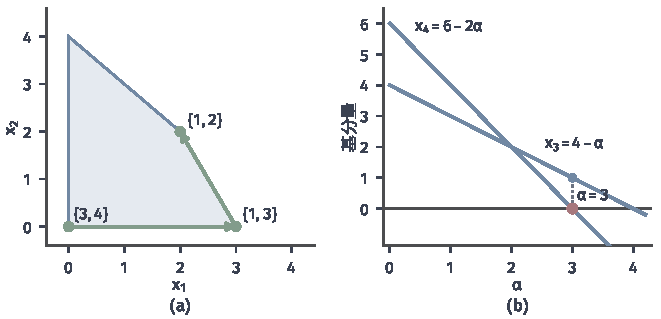
\includegraphics[width=112mm]{figures/05-optimization/01-linear-programming/matplotlib/lp-pivot-edge/figure.pdf}
 \caption{两次换基。(a)~绿色箭头沿边从$(0,0)$到$(3,0)$，再到$(2,2)$，点旁是当时的基。(b)~第一次移动时两个基分量随步长$\alpha$下降，$x_4$在$\alpha=3$处最先到零（红点），此时$x_3=1$。}
 \label{fig:lp-pivot-edge}
\end{BookInlineFigure}

\paragraph{含直线的多面体没有极点}
以上结论都是对标准型说的。它们能推广到什么范围？在平面上考虑带形
\[
 \{(x_1,x_2):0\leq x_2\leq1\}.
\]
最小化$x_2$，最优值$0$在整条直线$x_2=0$上取得，但这个集合没有角点。图~\ref{fig:lp-no-vertex-strip}(a)中，每个点都是左右两个可行点的中点。可见“有最优解就有最优顶点”不是所有多面体都有的性质，缺的是下面的秩条件。

\begin{BookInlineFigure}
 \centering
 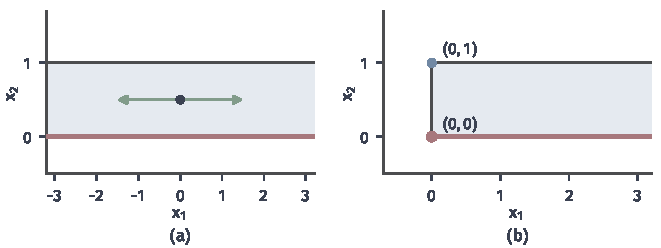
\includegraphics[width=112mm]{figures/05-optimization/01-linear-programming/matplotlib/lp-no-vertex-strip/figure.pdf}
 \caption{极点的存在依赖可行集的形状，目标取$x_2$，红色粗线是最优解集合。(a)~带形含有水平直线，绿色线段说明任一点都是两个可行点的中点，所以没有极点，最优解集合也没有端点。(b)~加上$x_1\geq0$后不再含直线，出现顶点$(0,0)$和$(0,1)$，最优值在顶点$(0,0)$取得。}
 \label{fig:lp-no-vertex-strip}
\end{BookInlineFigure}

\begin{lemma}[多面体的极点]
 \label{lem:lp-polyhedron-vertices}
 设$\bm{Q}=\{\bm{x}:\bm{G}\bm{x}\leq\bm{h}\}$非空，其中$\bm{G}$有$n$列。对$\bm{x}\in\bm{Q}$，记$I(\bm{x})$为取等号的行的下标集。则$\bm{x}$是极点，当且仅当$\bm{G}_{I(\bm{x}),:}$的秩为$n$。进一步，下面三条等价：$\bm{Q}$有极点；$\operatorname{rank}\bm{G}=n$；$\bm{Q}$不含直线。
\end{lemma}

\begin{proof}
 先证第一句。若取等号的行的秩小于$n$，存在$\bm{d}\neq\bm{0}$使这些行与$\bm{d}$的内积都为零。其余的行留有余量，$\varepsilon>0$足够小时$\bm{x}\pm\varepsilon\bm{d}\in\bm{Q}$，所以$\bm{x}$不是极点。反之设秩为$n$，且$\bm{x}=(\bm{u}+\bm{v})/2$，$\bm{u},\bm{v}\in\bm{Q}$。对每个$i\in I(\bm{x})$，两个不超过$h_i$的数平均后等于$h_i$，只能都等于$h_i$，所以$\bm{u}$和$\bm{v}$满足相同的取等号方程组。这个方程组的解唯一，故$\bm{u}=\bm{v}=\bm{x}$。

 再证三条等价。若$\operatorname{rank}\bm{G}<n$，取$\bm{d}\neq\bm{0}$使$\bm{G}\bm{d}=\bm{0}$，则过任一点沿$\bm{d}$的直线都在$\bm{Q}$中，这时由第一句也没有极点。反之若$\bm{Q}$含直线$\bm{x}+t\bm{d}$，则对全部$t\in\mathbb{R}$有$\bm{G}(\bm{x}+t\bm{d})\leq\bm{h}$，只能$\bm{G}\bm{d}=\bm{0}$，秩小于$n$。若有极点，由第一句$\bm{G}$的秩为$n$。

 剩下要证$\operatorname{rank}\bm{G}=n$时有极点。取$\bm{Q}$中使$\operatorname{rank}\bm{G}_{I(\bm{x}),:}$最大的点$\bm{x}$。假设这个秩小于$n$，取$\bm{d}\neq\bm{0}$与取等号的行都正交。由$\operatorname{rank}\bm{G}=n$，$\bm{G}\bm{d}\neq\bm{0}$，必要时换成$-\bm{d}$，可设有一行的内积为正。沿$\bm{d}$走到第一条新约束取等号为止，原来取等号的行仍取等号，新行与$\bm{d}$不正交，不在原来那些行的张成中，秩增大，矛盾。所以这个秩等于$n$，$\bm{x}$是极点。
\end{proof}

标准型中$\bm{G}$含有$-\bm{I}$这一块，秩一定是$n$，所以非负约束自动排除了直线。定理~\ref{thm:lp-optimal-bfs}成立的前提正是这一点。

上一节说自由变量分解会造出角点，这里可以看得很清楚。把带形写成标准型：令$x_1=x_1^{+}-x_1^{-}$，加松弛变量$w$，约束只剩一个等式$x_2+w=1$。基只能是$\{x_2\}$或$\{w\}$，基$\{w\}$给出的基本可行解$(x_1^{+},x_1^{-},x_2,w)=(0,0,0,1)$是最优的。它对应带形中的点$(0,0)$，这个点是最优解，却不是带形的顶点。所以应用定理时要分清：顶点是标准型的顶点，回到原问题后只保证是一个最优解。

\paragraph{退化基与无界可行方向}
基和点的对应还有两种偏差，表现相似，含义却不同，都发生在换基的时候。

第一种是几个基对应同一个点。给车间问题再加一条约束$x_1\leq3$，引入松弛变量$x_5$，得到$m=3$，$n=5$的标准型。可行域没有变化，但顶点$(3,0)$现在有三条边界经过，如图~\ref{fig:lp-degenerate-vertex}。这个点是
\[
 \bm{x}=(3,0,1,0,0)^\top,
\]
只有$x_1,x_3$两个正分量，而基需要三个下标。

\begin{BookInlineFigure}
 \centering
 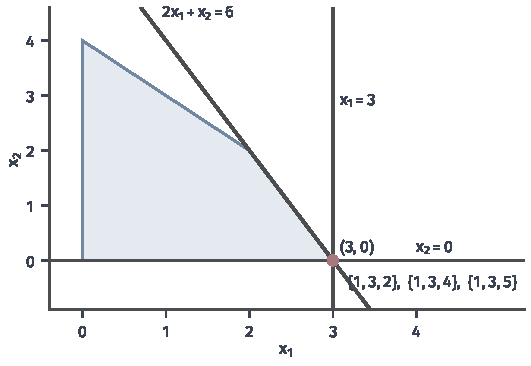
\includegraphics[width=90mm]{figures/05-optimization/01-linear-programming/matplotlib/lp-degenerate-vertex/figure.pdf}
 \caption{退化顶点。加入约束$x_1\leq3$后，四边形没有变，但三条深灰粗线同时经过红点$(3,0)$。第三个基下标取$2$、$4$或$5$，三个基$\{1,3,2\}$、$\{1,3,4\}$、$\{1,3,5\}$都给出这同一个点。}
 \label{fig:lp-degenerate-vertex}
\end{BookInlineFigure}

第三个下标可以取$2$、$4$或$5$，三个基矩阵都可逆，所以三个基给出同一个点，每个基中都有一个取零的基分量。这样的基称为\term{退化基}（degenerate basis），对应的基本可行解称为退化的。此时定理~\ref{thm:lp-edge-move}的条件$\bar{\bm{x}}_B>\bm{0}$不成立。

从基$\{1,3,2\}$（基分量依次为$3,1,0$）出发，让$x_4$增大，解$\bm{A}_B\bm{u}=\bm{a}_4$得到
\[
 \bm{u}=(0,-1,1)^\top,\qquad\alpha^\star=\frac{0}{1}=0.
\]
基变成$\{1,3,4\}$，点却一动不动。“换基”和“走到另一个顶点”在退化时不再是一回事。

第二种是沿某条边可以走到无穷远。取可行域$x_1-x_2\leq1$，$\bm{x}\geq\bm{0}$，写成标准型$x_1-x_2+x_3=1$，这里$m=1$。在基$\{3\}$处，点是$(0,0,1)^\top$。让$x_2$增大：
\[
 u=\bm{A}_B^{-1}\bm{a}_2=-1\leq0.
\]
由定理~\ref{thm:lp-edge-move}的情形2，沿$\bm{d}=(0,1,1)^\top$可以一直走。满足下面条件的$\bm{d}$称为\term{无界可行方向}（unbounded feasible direction）：
\begin{equation}
 \bm{A}\bm{d}=\bm{0},\qquad\bm{d}\geq\bm{0},\qquad\bm{d}\neq\bm{0}.
 \label{eq:lp-recession}
\end{equation}
任何可行点沿它走都不会离开$\bm{C}$。这是可行集形状的性质，与目标无关：可行集无界不等于问题无下界，只有$\bm{c}^\top\bm{d}<0$时目标才沿它趋于$-\infty$。图~\ref{fig:lp-three-outcomes}的(b)与(c)用的正是同一个可行域。表~\ref{tab:lp-degenerate-vs-ray}对比了这两种现象。

\begin{BookInlineTable}
 \centering
 \begin{tabular}{lll}
  \toprule
  & 退化基 & 无界可行方向 \\
  \midrule
  代数表现 & 基分量取零 & $\bm{u}\leq\bm{0}$ \\
  步长 & 可能$\alpha^\star=0$ & 没有上限 \\
  几何含义 & 多余约束过同一顶点 & 可行集沿射线无界 \\
  对目标的影响 & 换基后点和目标值不变 & $\bm{c}^\top\bm{d}<0$时无下界 \\
  \bottomrule
 \end{tabular}
 \caption{退化基与无界可行方向的对比。}
 \label{tab:lp-degenerate-vs-ray}
\end{BookInlineTable}
